\chapter{The Physics of Fire Remote
Sensing}\label{chapter-3-the-physics-of-wildfire-remote-sensing}

% \begin{quote}
% \textbf{Writing Guide \& Methodological Focus:}

% \begin{itemize}
% \item
%   \textbf{Objective:} To explain the fundamental science of \emph{how} a
%   fire can be "seen" from space. This chapter provides the physical
%   foundation for the sensor requirements and how they need to be
%   distributed over the constellation.
% \item
%   \textbf{Method:} Divide the physics into two parts: the source (the
%   fire) and the detection challenge (the observation).
% \item
%   \textbf{Caution:} Keep the physics focused and conceptual. Not
%   designing the sensor, but establishing the principles that dictate its
%   necessary characteristics.
% \item
%   \textbf{Checkpoint:} Does this chapter clearly explain \emph{why} a
%   satellite needs specific type of sensors to meet the
%   mission\textquotesingle s goals?
% \end{itemize}
% \end{quote}
The satellite constellation architecture configuration will depend on the distribution of satellite nodes across the orbital network and on the geometric constraints of each spacecraft's fire detectors. Therefore, the basic concept of fire remote detection from Earth orbit will be presented in this chapter to provide the necessary physical foundation for deducing mission requirements. 

\section{Physical Base of Remote Sensing}
\label{310-physical-base-of-remote-sensing}

A satellite sensor measures Electromagnetic (EM) energy within a given spectral band that reaches its aperture from a specific direction. This energy, reflected or emitted from a ground target, travels toward the detector. On this path, it interacts with the atmosphere, clouds, smoke, and other particles. The final energy flux measured will differ from the initial flux from the target due to these interactions. The fundamental radiometric quantity detected is the \textbf{radiance} $L$, defined below based on radiometric primitives.

\subsection{Radiometric primitives: irradiance, exitance, and radiance}
\begin{figure}
    \centering
    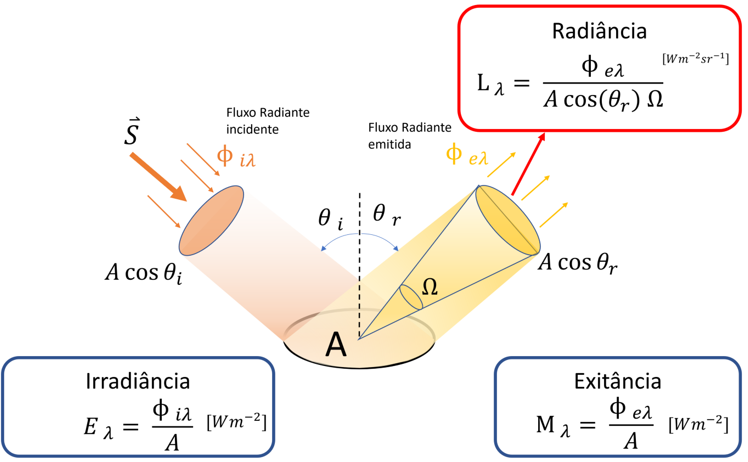
\includegraphics[width=0.75\linewidth]{images/remote_detection_principles.png}
    \caption{\footnotesize{Geometric definitions of the fundamental radiometric primitives. The diagram illustrates the distinction between the hemispherical fluxes of Irradiance ($E_\lambda$) and Exitance ($M_\lambda$), normalized by surface area $A$, versus the directional quantity of Radiance ($L_\lambda$), normalized by projected area $A \cos \theta_r$ and solid angle $\Omega$. Effects of atmospheric transmittance and path radiance are implicitly assumed in the propagation. }}
    \label{fig:remote_sense_radiometric_primitives}
\end{figure}

Consider the study domain $\mathcal{D}$ with a region target $\mathcal{R} \in \mathcal{F}_\oplus$ observed by a satellite as represented in Fig. \ref{fig:remote_sense_radiometric_primitives}. An elementary plane surface patch $S_j$, with $S_j \in \mathcal{R}$, has its area $A$ irradiated by electromagnetic radiation from the pointing vector $\vec{S}$ at an incidence angle $\theta_i$ with respect to the surface normal. Let $Q_{\lambda}$ be the radiant energy in a narrow spectral interval around wavelength $\lambda$ that crosses area $A$ within time $\Delta t$. The corresponding \textbf{spectral radiant flux} is
\begin{equation}
\phi_{\lambda} \;=\; \frac{Q_{\lambda}}{\Delta t}\quad [\mathrm{W}]\,.
\label{eq:spectral_radiant_flux}
\end{equation}
The incident flux per unit area is the \textbf{spectral irradiance} $E_{\lambda}$,
\begin{equation}
E_{\lambda} \;=\; \frac{\phi_{\lambda,i}}{A}\quad [\mathrm{W\,m^{-2}}] \,,
\label{eq:spectral_irradiance}
\end{equation}
while the flux \emph{leaving} the surface per unit area is the \textbf{spectral exitance} $M_{\lambda}$,
\begin{equation}
M_{\lambda} \;=\; \frac{\phi_{\lambda,e}}{A}\quad [\mathrm{W\,m^{-2}}] \;.
\label{eq:spectral_exitance}
\end{equation}
Radiance introduces directionality. The spacecraft detector at point $P_{sat}$, $P_{sat}(x^\mu)\footnote{We adopt General Relativity index notation (e.g., Carroll, \emph{Spacetime and Geometry}) for compactness, independent of the relativistic framework. Greek indices run $\mu=0,\dots,3$ (spacetime) and Latin indices $i=1,\dots,3$ (space). Thus, $x^\mu = (x^0, x^1, x^2, x^3) = (ct, x, y, z)$, with $t \in \mathcal{T}$ a temporal domain.} \in \mathcal{F}_{J2000}$, observes surface $S_j$ at the centralized target point $P_{target}$, $P_{target}(x^\nu) \in \mathcal{F}_{J2000}$, connected via the Line-of-Sight vector $\vec{r}_{LoS} = P_{target} - P_{sat}$. This instrument has a viewing direction that makes an angle $\theta_r$ with respect to the surface normal. The satellite detector, with an effective sensitive area $A_D$, collects the emitted radiant flux $\phi_{\lambda,e}$ over the solid angle $\Omega$. The \textbf{spectral radiance} measured by the detector is
\begin{equation}
L_{\lambda} \;=\; \frac{\phi_{\lambda,e}}{A\,\cos\theta_r\,\Omega}\quad [\mathrm{W\,m^{-2}\,sr^{-1}\,\mu m^{-1}}] \,.
\end{equation}

\subsubsection{From Radiance to Digital Number (DN)}
Satellites do not record radiance directly. Detectors convert incident photons into electric charge, which is quantized by an Analog-to-Digital Converter (ADC) into a discrete \textbf{Digital Number (DN)}. Recovering physical radiance requires radiometric calibration. While full sensor characterization is outside this work's scope, the process is generally approximated by a linear model for a spectral band $b$:
\begin{equation}
\mathrm{DN}_b \;\approx\; g_b\,L_{b,\mathrm{toa}} + o_b\,,
\end{equation}
where $g_b$ is the gain, $o_b$ the offset, and $L_{b,\mathrm{toa}}$ is the \textbf{Top-of-Atmosphere (TOA) band radiance}. Inverting this relation is the prerequisite for any physical interpretation of the fire scene.

\subsubsection{Radiance as a composition of reflective and emissive processes}
In a rigorous physical framework, spectral radiance is the superposition of multiple mechanisms: reflection, thermal emission, and secondary effects such as inelastic scattering (e.g., Raman) and luminescence. However, for the energy magnitudes involved in wildfire remote sensing, secondary quantum effects are negligible compared with solar reflection and thermal blackbody emission. Therefore, we approximate the surface radiance as a sum of two dominant components:
\begin{equation}
L_{\lambda,\mathrm{surf}} \;\approx\; L_{\lambda,\mathrm{refl}} + L_{\lambda,\mathrm{therm}}\,.
\end{equation}
The reflected component is driven by solar illumination and surface bidirectional reflectance (BRDF), while the thermal component is governed by temperature and emissivity (Planck's Law). A practical first-order forward model for what the satellite measures at TOA is:
\begin{equation}
L_{\lambda,\mathrm{toa}} \;=\; \tau_{\lambda}\,L_{\lambda,\mathrm{surf}} \; +\; L_{\lambda,\mathrm{path}}\,.
\end{equation}
Here $\tau_{\lambda}$ is the atmospheric transmittance along the line of sight and $L_{\lambda,\mathrm{path}}$ is the path radiance (scattering and atmospheric emission) added between the ground and the sensor. Transmittance is the superposition of terms:
\begin{equation}
\tau_{\lambda} \;\approx\; \tau_{\lambda,\mathrm{gas}}\,\tau_{\lambda,\mathrm{aer}}\,\tau_{\lambda,\mathrm{smoke}}\,\tau_{\lambda,\mathrm{cloud}}\,,
\label{eq:tranmitance_atm}
\end{equation}
where the last two terms highlight how \textbf{smoke} and \textbf{cloud} can severely attenuate the signal. These terms are treated in Sec.~\ref{subsec:atmospheric_limit} in the context of observability constraints.
\paragraph{The limit of Reflectance products for Fire detection.}
Many Earth Observation products are reported as a radiance-normalized surface reflectance ($\rho_\lambda$), intuitively defined as the ratio of exiting flux to incoming flux:
\begin{equation}
\rho_{\lambda} \;= \frac{M_\lambda}{E_\lambda} \;\approx\; \frac{\pi\,L_{\lambda,\mathrm{surf}}}{E_{\lambda,\mathrm{down}}\,\cos\theta_i}\quad (\text{Lambertian approx.})\,.
\end{equation}
For standard land cover, this approximation holds because the upwelling radiance is dominated by reflection ($L_{\lambda,\mathrm{surf}} \approx L_{\lambda,\mathrm{refl}}$). However, active fires break this intuition. For a fire pixel, the surface is not only reflecting sunlight but is also \emph{actively emitting} intense thermal radiation ($L_{\lambda,\mathrm{therm}}$). 

If one were to apply the standard reflectance formulation and calibration with sun light as reference to a fire pixel, the additional term $L_{\lambda,\mathrm{therm}}$ would result in a mathematically valid but physically misleading "reflectance" value (often $> 1.0$). Consequently, fire characterization cannot rely on passive reflective metrics. Instead, it requires isolating the thermal excess to quantify the energy release by the combustion of the material. This necessitates a dedicated metric: \textbf{Fire Radiative Power (FRP)}. 

FRP provides a direct quantitative link to the amount of biomass consumed (combustion rate) and the intensity of the fire front. 

\section{The Fire Itself: Physics of the Radiative Signature}
\label{31-the-fire-itself-physics-of-the-radiative-signature}

This chapter establishes the physical foundation linking the thermal emission of a wildfire to the digital signal received by a satellite. We transition from the theoretical laws of blackbody radiation to the operational metric of Fire Radiative Power (FRP), which quantifies the rate of radiant energy release from a fire. This framework is key as it redefines "detection" from a binary flag to a quantitative threshold based on fire intensity, allowing validation against FIRMS fire records.

\subsection{The Operational Standard: FRP used in FIRMS Dataset}
In this constellation design study, the objective is not merely to detect a "hotspot" but also to quantify detection performance against realistic fire intensities and to avoid false positives (e.g., industry, clouds, and IR reflection artifacts). To achieve this, we adopt Fire Radiative Power (FRP) as the fundamental metric for fire characterization \inlineReq{R26}.

FRP, measured in MegaWatts [MW], is the standard variable in global fire inventories; it is used in the Fire Information for Resource Management System (FIRMS) described in section \ref{sec:firms_dataset}. The algorithms described in this section are used to generate the FIRMS geostationary fire datasets, serving as a validation reference in later simulations. Each satellite node in the constellation will be evaluated on its ability to detect historical fire events, based on its statistical FRP values from these principles, as shown here.

\subsection{The Spectral Signature of Fire}
\label{311-the-spectral-signature-of-fire}

The derivation of FRP starts with blackbody radiation physics. A fire emits energy across the spectrum, but satellites measure radiance only in specific bands. To estimate total energy, we use the Stefan-Boltzmann Law. This section is base on Wooster et al. work \cite{wooster_retrieval_2005}.

\subsubsection{Fire Radiative Power Theoretical Foundation}
Any object with a physical temperature $T > 0$ K emits electromagnetic radiation. The total power emitted per unit area, defined as the \textbf{radiant exitance} $M$, is governed by the Stefan-Boltzmann Law:
\begin{equation}
    M \;=\; \varepsilon \sigma T^4 \quad [\mathrm{W\,m^{-2}}]
\end{equation}
where $\sigma$ is the Stefan-Boltzmann constant ($5.67 \times 10^{-8}\,\mathrm{W\,m^{-2}\,K^{-4}}$), and $\varepsilon$ is the emissivity ($0 \leq \varepsilon \leq 1$), representing the efficiency of the emitter compared to a perfect blackbody.

For a fire occupying a surface area $A_{fire}$ with an effective temperature $T_{fire}$, the total \textbf{Fire Radiative Power (FRP)} is the integral of this exitance over the active flaming area:
\begin{equation}
    FRP \;=\; \int_{A_{fire}} M \, dA \;\approx\; A_{fire} \cdot \varepsilon_{fire} \cdot \sigma \cdot T_{fire}^4 \quad [\mathrm{W}]
    \label{eq:frp_integral_problem}
\end{equation}
This equation represents the "ground truth" energy release we wish to measure. However, solving Eq. \ref{eq:frp_integral_problem} directly is impossible for a satellite sensor because:
\begin{enumerate}
    \item The sensor does not measure the total bolometric spectrum ($M$); it measures radiance in specific narrow bands (e.g., MIR at $3.8\mu$m).
    \item The fire area $A_{fire}$ is typically much smaller than the pixel size ($A_{fire} \ll A_{pixel}$), making it an unresolved sub-pixel feature with an unknown effective temperature $T_{fire}$.
\end{enumerate}

\subsubsection{The Middle-Infrared (MIR) Radiance Method}
To bypass the need for resolving $A_{fire}$ and $T_{fire}$ explicitly, modern operational algorithms (MODIS, VIIRS, FIRMS) use the \textbf{MIR Radiance Method} (Wooster et al., 2003)\cite{wooster_fire_2003}. This method relies on a physical coincidence: in the Middle-Infrared (MIR) spectral window ($\sim 3.8 \mu$m), the Planck function $B(\lambda, T)$ approximates a fourth-order power law for the temperature range of active fires ($600\,\mathrm{K} - 1300\,\mathrm{K}$).

The fire-emitted spectral radiance $L_{f,MIR}$ can therefore be approximated as:
\begin{equation}
    L_{f,MIR} \;=\; \varepsilon_{f,MIR} B(\lambda, T_{fire}) \;\approx\; \varepsilon_{f,MIR}\, a \, T_{fire}^4 \propto M
    \label{eq:mir_power_law}
\end{equation}
where $a$ is a sensor-specific constant (units $\mathrm{W\,m^{-4}\,sr^{-1}\,\mu m^{-1}\,K^{-4}}$).

\paragraph{Deriving FRP without Temperature.}
Crucially, the power law in Eq. \ref{eq:mir_power_law} is identical in form to the Stefan-Boltzmann law ($M \propto T^4$). By equating these two relations, we can isolate $T^4$ and substitute it back into the FRP definition.

From Eq. \ref{eq:mir_power_law},  we can find the fire temperature T:
\begin{equation}
T_{fire}^4 \approx \frac{L_{f,MIR}}{a \cdot \varepsilon_{f,MIR}}
\label{eq:Temperature_from_radiance}
\end{equation}
Substituting this into the FRP equation:
\begin{equation}
    FRP \;=\; A_{fire} \cdot \varepsilon_{fire} \cdot \sigma \cdot \left( \frac{L_{f,MIR}}{a \cdot \varepsilon_{f,MIR}} \right)
\end{equation}

Assuming the fire behaves as a gray body ($\varepsilon_{fire} \approx \varepsilon_{f,MIR}$), the emissivity terms cancel out. Furthermore, the term $A_{fire} \cdot L_{f,MIR}$ is simply the total spectral intensity measured by the satellite pixel (Fire Spectral Radiance $\times$ Area). This yields the fundamental result:
\begin{equation}
    FRP \;=\; \left( \frac{\sigma}{a} \right) L_{f,MIR}^{tot}
\end{equation}
This implies that the total fire radiative power is directly proportional to the fire's MIR radiance, independent of its specific temperature or sub-pixel area. Also, the fire temperature T can be found by inverting FRP to get $L_{f,MIR}$, and using equation \ref{eq:Temperature_from_radiance}. This temperature connects to the biomass combustion rate.

\subsubsection{The Operational Equation}
Based on this derivation, the operational equation used to retrieve FRP in the FIRMS dataset is (Wooster et al., 2015)\cite{wooster_lsa_2015}:

\begin{equation}
    FRP_{pixel} \;=\; \frac{A_{pixel} \cdot \sigma}{a \cdot \tau_{MIR}} \left( L_{MIR} - L_{MIR, bg} \right) \quad [\mathrm{MW}]
    \label{eq:frp_operational}
\end{equation}

Where, $A_{pixel}$ represents the ground projection area of the satellite pixel, and $\sigma$ denotes the Stefan-Boltzmann constant. The parameter $a$ is the sensor-specific empirical power-law constant (approx. $3.0 \times 10^{-9}$ for MODIS), while $\tau_{MIR}$ accounts for atmospheric transmittance. The final term, $(L_{MIR} - L_{MIR, bg})$, isolates the active fire signal by subtracting the ambient background radiance. As FIRMS comprises 5 sensors, it uses distinct versions of the FRP methods. They are based on a Geostationary Fire Thermal Anomaly (FTA) algorithm and FRP retrieval developed by King’s College. which are discussed in the following articles: \cite{davies_geostationary_2024a}, \cite{hall_validation_2019}, \cite{roberts_fire_2008}
\begin{figure}[H]
    \centering
    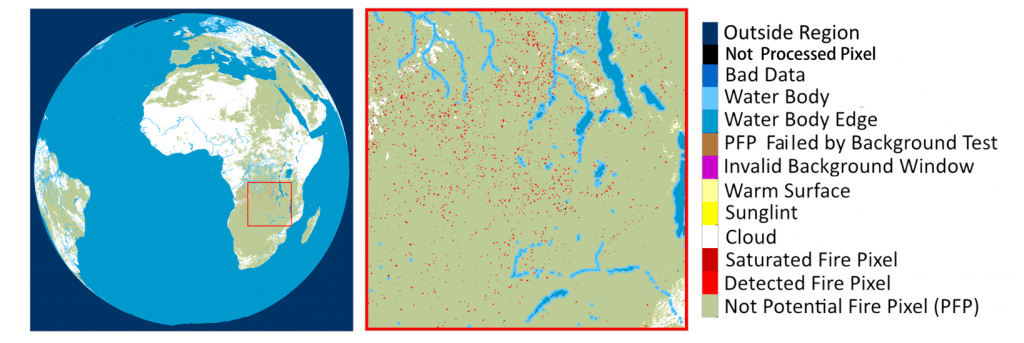
\includegraphics[width=1\linewidth]{images/Meteosat_FRP_pixels.png}
    \caption{\footnotesize{Example Meteosat SEVIRI FRP-PIXEL Product example, derived from SEVIRI imagery collected at 13:00 UTC on 5\textit{th}\textit{ July 2015}. Meteosat is one of the geostationary sensors from FIRMS.\cite{_access_kings_wildfire}}}
    \label{fig:Meteosat_FRP_pixels}
\end{figure}
\subsubsection{Confidence of Fire Event Detection}

To minimize false positives in the validation dataset, we enforce strict classification boundaries: a minimum Fire Radiative Power of $FRP_{min} = 50\,\mathrm{MW}$ and a \textbf{Confidence Level of 100\%} \inlineReq{R27}. In the FIRMS algorithm, confidence is a metric from detection data (e.g., anomaly strength, sun glint potential). Choosing "High Confidence" (100\%) pixels filters the dataset to events with saturated readings or strong anomalies (>15K), removing sun glint, weak signals, and ambiguous detections.s detections\cite{earthsciencedatasystems_viirs_2024}.


\subsection{Key Multi-spectral Bands for Broad Fire Analysis}
\label{312-key-spectral-bands-for-fire-analysis}

To satisfy mission requirements for fire resilience \reqRef{R1}, ignition anticipation \reqRef{R2}, and all-weather capability \reqRef{R5}, a comprehensive mission would  need a diverse multispectral payload:

\begin{itemize}
    \item \textbf{Visible (VIS):} Essential for tracking smoke plume dynamics, distinguishing clouds from smoke, and providing intuitive geographic context for ground teams.
    \item \textbf{Near-Infrared (NIR):} Key for assessing vegetation health (fuel load estimation) and mapping post-fire burn scars.
    \item \textbf{SWIR:} Identifies high-temperature anomalies and moisture contrast (discriminating hot ground from warm smoke).
    \item \textbf{MWIR \& LWIR:} The primary bands for active heat detection, temperature retrieval, and FRP calculation.
    \item \textbf{SAR:} Enables all-weather biomass mapping and fire line detection through thick smoke and clouds (structural change detection).
\end{itemize}

However, detailed instrument optimization is outside the scope of this geometric analysis. We leave detailed instrument design tradeoffs for future research. For this study, we assume standard detection capabilities based on the FRP principles described  \inlineReq{R28}. This assumption is robust for the core study domain, as most fire seasons occur during hot, cloud-free periods.

It is important to recognize that this approach relies on optical visibility. Specific operational scenarios, such as mega-fire events with high smoke density, tropical cloud cover, or coastal regions where diurnal fog obscures morning hotspots (e.g., the Portuguese coast), would require the SAR or multispectral capabilities mentioned to maintain continuity, early detection, and effective fire combat. SAR is also a prominent new technology for combating fires in tropical forests, which are very often obscured by dense clouds. These instrumentation trade-offs are reserved for future research; the current focus remains on the satellite network geometry, the sensors' field of view, and the spacecraft system's coverage.

%%%%%%%draft
\section{Sensor Observation Constraints}
\label{sec:sensor_observation_constraints}

The temporal resolution performance of a constellation is driven by the revisit time $t_{rev \to P_j}$ to a target $P_j$. The revisit frequency depends on the trade-off between the network's satellite density and the duration and quality of each pass, which are governed by the individual sensor's geometric and optical limits.

The detailing constellation observation formalism connected with orbital dynamics is discussed in the Methodology (Chapter \ref{sec:Constellation_observation_form}). Before this details, to limit the scope of work, we must first define the physical limits of the atmosphere which will lead to observation constraints. A valid detection event is not merely a line-of-sight problem; it requires the signal quality of the intersection of two distinct geometric volumes: the \textbf{Ground Access Window} (the ground target's view of the sky) and the \textbf{Space Access Window} (the satellite's view of the ground), as shown in Fig \ref{fig:access_nominal_and_limit}.

\subsection{Physical Limit: Atmospheric Attenuation}
\label{subsec:atmospheric_limit}
As discussed in the Radiance Chapter, the infrared signal is modulated by the atmospheric transmittance $\tau_\lambda$ (Eq. \ref{eq:tranmitance_atm}). Factors such as clouds, smoke aerosols, and water vapor significantly attenuate the signal.

Observations at low elevation angles $\varepsilon$ (near the horizon) traverse a much thicker atmospheric layer compared to the Zenith path, drastically degrading the Signal-to-Noise Ratio (SNR). The path length through the atmosphere scales with $\approx 1/\sin(\varepsilon)$. 

To mitigate these effects without performing complex real-time radiative transfer modelling, we impose a strict geometric constraint. We define the operational limits: the \textbf{Minimum Elevation Angle} $\varepsilon_{min} = 15^\circ$, \inlineReq{R29}, and \textbf{Maximium Athmospheric grazing angle} $\theta{\text{atm max}}=65^\circ$, \inlineReq{R30}. 

This threshold acts as a proxy for signal quality, filtering out observations where transmittance is likely to be dominated by scattering and absorption.

\subsection{Geometric Access Windows}
Based on the physical limit defined above, we construct two geometric volumes that define the valid observation space, as illustrated in Fig. \ref{fig:access_nominal_and_limit}.

\begin{figure}[H]
    \centering
    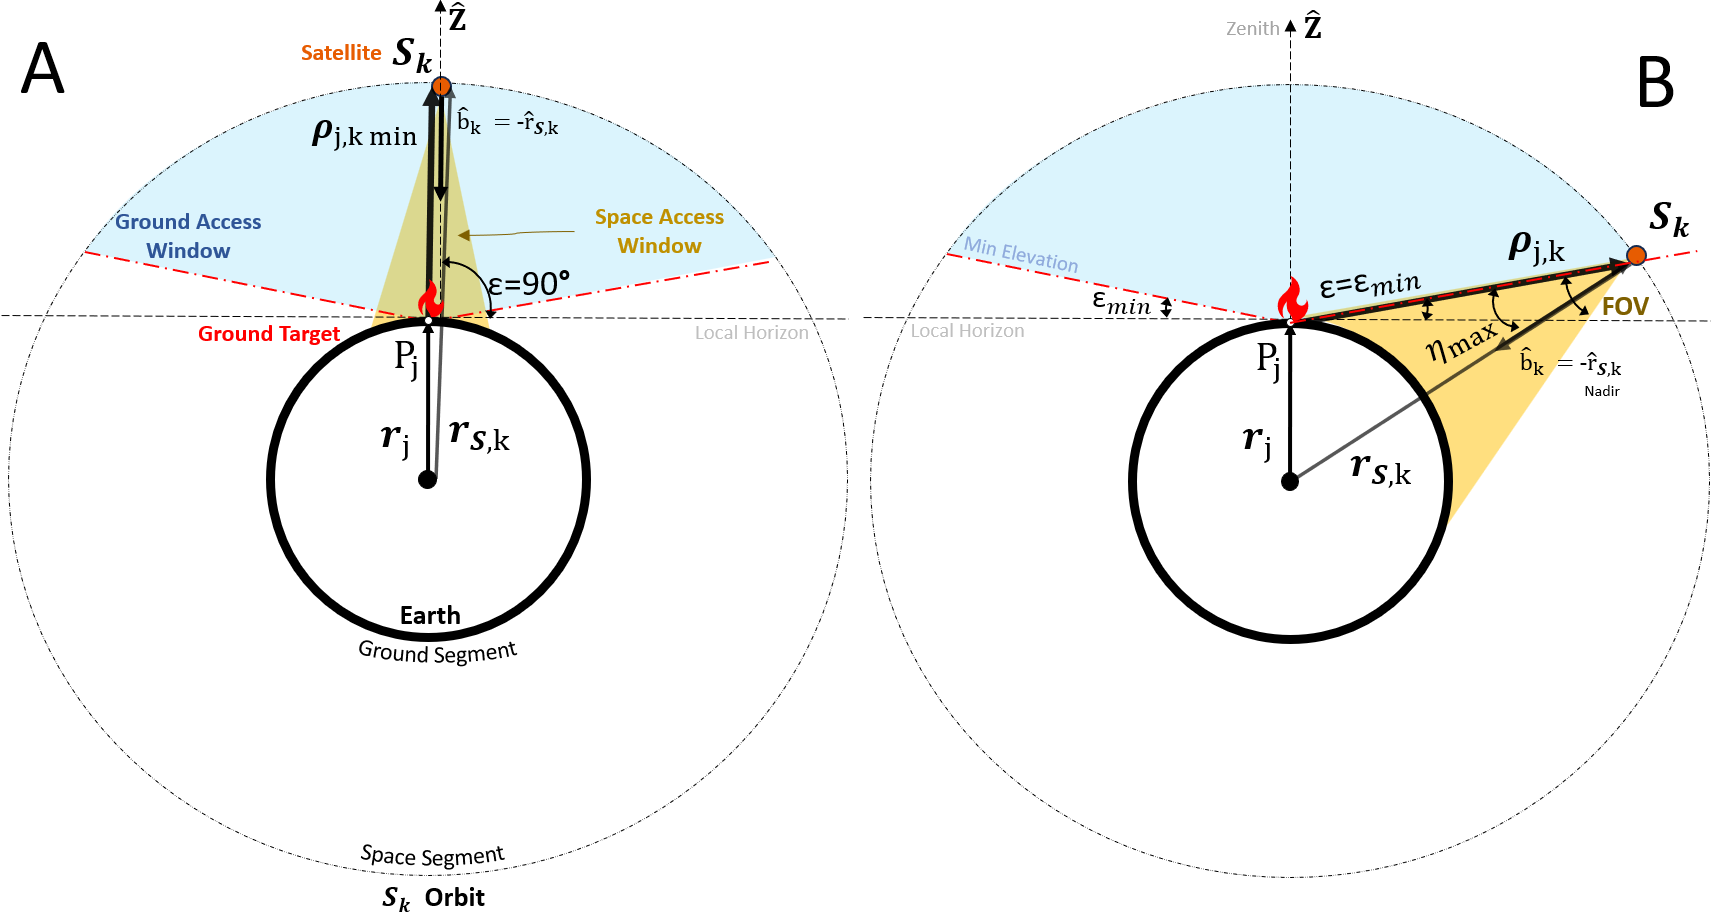
\includegraphics[width=1\linewidth]{images/access_nominal_and_limit.png}
    \caption{\footnotesize{Geometric definition of the Observation Constraints. The valid detection volume is formed by the intersection of the Ground Access Window (Blue) and the Space Access Window (Yellow). A) Highlights the Nominal Zenith case (best quality) where ground resolution GSD is calculated. B) Visibility limit configuratrion, edge of the coverage where Ground \& Space Access windows meet ($\epsilon_{min}$ and $\eta_{max}$).}}
    \label{fig:access_nominal_and_limit}
\end{figure}

\subsection{Ground Access Window ($\mathcal{W}_{ground}$)}
The Ground Access Window $\mathcal{W}_{ground,j}$ represents the volume of the local sky physically visible and useful to the target point $P_j$. While a target theoretically has a $180^{\circ}$ view of the sky (from horizon to horizon), practical observation is limited by terrain geometric masking and atmospheric attenuation.

We define the constraint using the \textbf{Elevation Angle $\varepsilon$}, measured from the local horizon to the satellite. To ensure valid data retrieval, the satellite must be above a minimum elevation threshold:
\begin{equation}
    \mathcal{W}_{ground,j} = \{ \text{Visible} \mid \varepsilon \geq \varepsilon_{min} \}
\end{equation}
For this mission analysis, as discussed, we set the requirement to $\varepsilon_{min} = 15^{\circ}$. Below this angle, the path length through the atmosphere increases drastically, degrading the signal-to-noise ratio and geometric accuracy.

\subsection{Space Access Window ($\mathcal{W}_{space}$)}
The Space Access Window represents the conical volume observable by the spacecraft $S_k$. This volume encloses all potential instrument architectures (e.g., push-broom scanners, matrix cameras) and is defined relative to the satellite's Sensor Boresight Vector $\hat{\mathbf{b}}_k$, which nominally points toward the geodetic Nadir.

We define the constraint using the \textbf{Off-Nadir Angle $\eta$}, measured from the boresight vector $\hat{\mathbf{b}}_k$ to the the Relative Position Vector $\vec{\rho}_{j,k}$ between ground target $P_j$ and the satellite $S_k$. The limit is determined by the maximum reachable angle of the spacecraft optical system:
\begin{equation}
    \mathcal{W}_{space} = \{ \text{Visible} \mid \eta \leq \eta_{max} \}
\end{equation}
For a standard Earth-observation missions (LEO-MEO), achieving the good quality optical signal typically demands a maximum off-nadir view of $\eta_{max} = \theta{\text{atm max}} \approx 65^{\circ}$, \inlineReq{R31}. This cone defines the max Full Field of View for the satellites, \inlineReq{R32}.
\begin{equation}
    FOV = 2  \eta_{max} = 130^\circ; 
\end{equation}
\subsection{The Visibility Condition}
Consequently, a fire event at $P_j$ is only detected when the satellite enters the intersection of these two windows as shown in Fig \ref{fig:access_nominal_and_limit}-B. The geometric requirement for observation is the simultaneous satisfaction of both access windows angular constraints\inlineReq{R33}:

\begin{equation}
    \text{Observation Link} \ \mathcal{L}_{j,k} \iff Visible
    \begin{cases} 
        \varepsilon \geq 15^{\circ} & \text{(Ground access: clear sky horizon)} \\
        \eta \leq 65^{\circ} & \text{(Space access : sensor athmospheic gazing limit)}
    \end{cases}
\end{equation}

\subsection{Optical Quality: Ground Sample Distance (GSD)}
\label{optical-quality}
The spatial resolution of the detected fire is governed by the \textbf{Ground Sample Distance (GSD)}. For this constellation design analysis we have the spacecraft at the nadir configuration as shown in Fig \ref{fig:access_nominal_and_limit}-A. On this observation setting, we utilize the first-order paraxial approximation calculated at nadir, \inlineReq{R34}. The GSD is deffined in function of the satellite altitude $h(t) = \|  \vec{\rho}_{j,k}  \|$:
\begin{equation}
    \text{GSD}(t) \approx \frac{p \cdot h[n]}{f}
    \label{eq:gsd}
\end{equation}
where $p$ is the detector pixel pitch and $f$ is the effective focal length. Athmospheric effects is not taking in consideration. 

\paragraph{Simulation Parameters:}
For the specific instrument modeled in this thesis, we assume the following optical characteristics:
\begin{itemize}
    \item Pixel Pitch: $p = 12um $ 
    \item Focal Length: $f = 600mm$ 
\end{itemize}

\paragraph{High-Fidelity Simulation Requirements.}
It is important to note that this linear approximation represents the "best-case" scenario. It does not account for off-nadir distortion where GSD degrades, optical aberrations, or motion smear. A rigorous validation of these parameters requires end-to-end optical simulation using Fourier optics tools (e.g., \textbf{Zemax OpticStudio}) and ruggedized geolocation libraries (e.g., \textbf{Rugged}), \cite{segl_s2etes_2015}, \cite{alici_image_2019}, \cite{_rugged_}. 

\section{Daily Fire-Behavior Temporal Observation Requirements}
\label{sec:_fire_daily_temporal_requirements}

Fires exhibit diurnal behavior driven by the daily evolution of atmospheric conditions, solar irradiance, temperature, relative humidity, and wind speed. This cycle is characterized by the temporal profiles of \textbf{Fire Radiative Power (FRP)}. Different types of sensors may be needed to investigate this variable temporal response, but they are out of scope, as discussed in section \ref{312-key-spectral-bands-for-fire-analysis}. However, we still need a "peak-fire hour" to synchronize the constellation at the $t_{\text{peak fire ref day}} = \text{ August 18th}$ at Coimbra, described in \reqRef{R16}.

Generally, the daily fire cycle has a spectrum of radiance that follows a loop relative to solar irradiation:
\begin{enumerate}
    \item \textbf{Smoldering Phase (Night/Early Morning, $\sim$00:00--09:00):} Higher humidity and lower temperatures suppress combustion, often reducing fires to a smoldering state (low FRP).
    \item \textbf{Growth Phase (Late Morning, $\sim$09:00--13:00):} Solar heating breaks the nocturnal pattern, lowering humidity and increasing wind mixing, causing a rapid ramp-up in FRP.
    \item \textbf{Peak Intensity (Afternoon, $\sim$13:00--18:00):} The coincidence of maximum temperature and wind speeds drives the fire to its maximum radiative output.
    \item \textbf{Decay Phase (Evening, $\sim$18:00--23:00):} As solar forcing vanishes, the boundary layer stabilizes, and intensity gradually declines.
\end{enumerate}

\subsection{Operational Windows for Portugal}
In Portugal, correlating peak fire activity with the diurnal temperature maximum (typically 13:00--15:00) can be misleading. The region is strongly influenced by strong Atlantic oceanic winds (e.g., the Nortada), which often intensify in the afternoon, decoupling peak fire intensity from peak solar irradiance. While a rigorous historical analysis of past fire events is necessary to precisely calibrate sensor timing for specific micro-climates, this study prioritizes aligning the constellation's orbit to intercept the estimated \textbf{maximum FRP peak at approximately 15:00 Local Time at Coimbra}, \inlineReq{R35}. 

\begin{equation}
    t_{\text{peak fire ref hour}} = \text{ 15:00 Local Time @ Coimbra }
    \label{eq:peak_fire_ref_hour}
\end{equation}


\section{Requirements of Fire Observation
Summary}\label{33---requirements-of-fire-observation-summary}

This section consolidates the fire remote-sensing constraints derived in the preceding sections into traceable, design-level requirements. These requirements establish the radiometric detection standard, the geometric observation boundaries, the optical resolution model, and the temporal synchronization reference for the constellation simulation. The requirements are organized into four categories: Fire Characterization, Sensor Observation Geometry, Optical Quality, and Temporal Observation.


Detailed requirements derived in this chapter (R26--R35), including Fire Characterization, Sensor Observation Geometry, Optical Quality, and Temporal Observation, are provided in Appendix~\ref{sec:app_req_ch3}.